\documentclass{article}

% Import packages from local file
\usepackage{packages}

% Define the homework number as a variable
\newcommand{\HomeworkNumber}{6}

\begin{document}

% Add the cover


% Set up custom date format
\newdateformat{monthyeardate}{\monthname[\THEMONTH] \THEYEAR}

% Header and Footer configuration
\pagestyle{fancy}
\fancyhf{}
\fancyhead[L]{\leftmark}
\fancyhead[R]{\thepage}
\fancyfoot[C]{Probabilistic Modeling and Reasoning Homework \HomeworkNumber}

% Chapter and Section formatting
\titleformat{\chapter}[display]
  {\normalfont\bfseries}{}{0pt}{\Huge}
\titlespacing*{\chapter}{0pt}{-20pt}{20pt}

% Adjust header height and top margin
\setlength{\headheight}{14.49998pt}
\addtolength{\topmargin}{-2.49998pt}

% Custom abstract environment
\newenvironment{customabstract}
  {\vspace*{1cm}
   \begin{center}
   \bfseries \huge Abstract
   \end{center}
   \vspace{0.5cm}
   \normalfont \large}
  {\vspace{1cm}}



\makeatletter
% Taken from http://ctan.org/pkg/centernot
\newcommand*{\centernot}{%
  \mathpalette\@centernot
}
\def\@centernot#1#2{%
  \mathrel{%
    \rlap{%
      \settowidth\dimen@{$\m@th#1{#2}$}%
      \kern.5\dimen@
      \settowidth\dimen@{$\m@th#1=$}%
      \kern-.5\dimen@
      $\m@th#1\not$%
    }%
    {#2}%
  }%
}
\makeatother


\begin{titlepage}
    \centering

    % University logo
    \vfill
    
\includegraphics[width=0.3\textwidth]{UOMLOGOEN.eps}
    \vfill

    % Main title
    {\Huge \textbf{Probabilistic Modeling and Reasoning}} \\
    {\LARGE Homework — \HomeworkNumber}

    \vfill  % Vertical fill for dynamic centering
    % Authors' names
    {\Large \textbf{Nikolaos Liouliakis (AID25001)}} \\
    {\Large \textbf{Vasileios-Efraim Tsavalia (AID25006)}}

    % \vfill

    % % Course submission information
    % {\Large A report submitted for the course} \\
    % {\Large \textbf{Probabilistic Modeling and Reasoning}}

    \vfill

    % Program and University information
    {\Large MSc in Artificial Intelligence and Data Analytics} \\
    {\Large University of Macedonia}

    \vfill


    % Supervisor information
    {\Large \textbf{Supervisor: Professor Dimitris Christou-Varsakelis}}

    \vfill

    % Date with custom format
    {\Large \monthyeardate\today} % Automatically displays in "October 2024" format
    
\end{titlepage}


\newpage



\section*{Problem 1}

The model selection was implemented in the \textit{P1\_coin\_tossing.m} MATLAB script. 
To overcome numerical issues for large values of \(N_{\text{Heads}}\) and \(N_{\text{Tails}}\) the Log-Sum-Exp trick was used.


\subsection*{1. Direct Approach}
The direct approach calculates the Bayes factor by summing terms involving high powers and small probabilities:
\[
p_{\text{Data}|\text{Model}_i} = \sum \theta^{N_{\text{Heads}}} (1-\theta)^{N_{\text{Tails}}} \cdot \text{pdf}_i(\theta)
\]
This approach works for the special case when $\theta = 0$ or $1-\theta = 0 $ and $N_{\text{Heads}}=0$ or $N_{\text{Tails}}=0$ respectively because in MATLAB  $0 ^ 0 = 1$, avoiding undefined behavior. However, it can still suffer from underflow when probabilities (\(\theta\) or \(1-\theta\)) are raised to large powers (\(N_{\text{Heads}}\), \(N_{\text{Tails}}\)).

\subsection*{2. Logarithmic Approach}
The logarithmic approach mitigates underflow and precision issues by:
\begin{enumerate}
    \item Computing the log of each term:
    \[
    \log(\text{term}) = N_{\text{Heads}} \cdot \log(\theta) + N_{\text{Tails}} \cdot \log(1-\theta) + \log(\text{pdf}_i(\theta))
    \]
    \item Using the \texttt{logsumexp} trick to sum terms in log-space:
    \[
    \log\left(\sum \text{terms}\right) = c + \log\left(\sum \exp\left(\log(\text{terms}) - c\right)\right)
    \]
    where \(c = \max(\log(\text{terms}))\) ensures numerical stability.
    \item Finally, converting the log-ratio back to linear scale:
    \[
    \text{Bayes Factor (accurate)} = \exp\left(\log(p_{\text{Data}|\text{Model}_1}) - \log(p_{\text{Data}|\text{Model}_2})\right)
    \]
\end{enumerate}

This method avoids the pitfalls for the special cases mentioned above, as MATLAB handles \texttt{0 * \(\infty\) = NaN} gracefully using \texttt{omitnan} during summation.


\section*{Problem 2}

The given linear model is:
\[
y_{t+1} = \sum_{k=1}^{K} w_k x_{t,k} = \mathbf{w}^\top \mathbf{x}_t,
\]
where:
\begin{itemize}
    \item $\mathbf{x}_t$ is the vector of features (factors) on day $t$,
    \item $\mathbf{w}$ is the vector of weights to estimate,
    \item $\mathbf{D} = \{(\mathbf{x}_t, y_{t+1})\}_{t=1}^{T-1}$ is the historical data,
    \item $\sigma_t^2$ represents the volatility for each day.
\end{itemize}

The returns $y_t$ are assumed to follow a Gaussian distribution. The likelihood is:
\[
p(y_{1:T} | \mathbf{x}_{1:T}, \mathbf{w}) = \prod_{t=2}^T \mathcal{N}\left(y_t | \mathbf{w}^\top \mathbf{x}_{t-1}, \sigma_t^2\right),
\]
which expands to:
\[
p(y_{1:T} | \mathbf{x}_{1:T}, \mathbf{w}) = \prod_{t=2}^T \frac{1}{\sqrt{2\pi \sigma_t^2}} \exp\left(-\frac{(y_t - \mathbf{w}^\top \mathbf{x}_{t-1})^2}{2 \sigma_t^2}\right)
\]

\subsection*{a)}
\subsubsection*{Log-likelihood}
Taking the log of the likelihood:
\[
\log p(y_{1:T} | \mathbf{x}_{1:T}, \mathbf{w}) = \sum_{t=2}^T \left[ -\frac{1}{2} \log(2\pi \sigma_t^2) - \frac{(y_t - \mathbf{w}^\top \mathbf{x}_{t-1})^2}{2 \sigma_t^2} \right].
\]

Ignoring the term $-\frac{1}{2} \log(2\pi \sigma_t^2)$ (independent of $\mathbf{w}$), the negative log-likelihood (NLL) becomes:
\[
\text{NLL}(\mathbf{w}) = \frac{1}{2} \sum_{t=2}^T \frac{(y_t - \mathbf{w}^\top \mathbf{x}_{t-1})^2}{\sigma_t^2}.
\]

\subsubsection*{Objective function for maximum likelihood}
Maximizing the likelihood is equivalent to minimizing the NLL:
\[
\mathbf{w}^* = \arg \min_{\mathbf{w}} \frac{1}{2} \sum_{t=2}^T \frac{(y_t - \mathbf{w}^\top \mathbf{x}_{t-1})^2}{\sigma_t^2}.
\]

\subsubsection*{Gradient of the NLL}
Expanding the quadratic term:
\[
\text{NLL}(\mathbf{w}) = \frac{1}{2} \sum_{t=2}^T \frac{1}{\sigma_t^2} \left[ y_t^2 - 2 y_t (\mathbf{w}^\top \mathbf{x}_{t-1}) + (\mathbf{w}^\top \mathbf{x}_{t-1})^2 \right].
\]

\[
\text{NLL}(\mathbf{w}) = \frac{1}{2} \sum_{t=2}^T \frac{1}{\sigma_t^2} \left[ y_t^2 - 2 y_t \mathbf{x}_{t-1}^\top \mathbf{w} + \mathbf{w}^\top \mathbf{x}_{t-1} \mathbf{x}_{t-1}^\top  \mathbf{w} \right].
\]



The gradient with respect to $\mathbf{w}$ is:
\[
\frac{\partial \text{NLL}(\mathbf{w})}{\partial \mathbf{w}} = -\sum_{t=2}^T \frac{y_t}{\sigma_t^2} \mathbf{x}_{t-1}^\top + \sum_{t=2}^T \frac{\mathbf{x}_{t-1} \mathbf{x}_{t-1}^\top }{\sigma_t^2} \mathbf{w}
\]

Let 
\[ \mathbf{A_1}  =  \sum_{t=2}^T \frac{\mathbf{x}_{t-1} \mathbf{x}_{t-1}^\top }{\sigma_t^2} \]

\[\mathbf{b_1} = \sum_{t=2}^T \frac{y_t}{\sigma_t^2} \mathbf{x}_{t-1}^\top  \]

The solution/maximum likelihood estimate for $\mathbf{w}$ is:

\[
\mathbf{w} = \mathbf{A_1}^{-1} \mathbf{b}
\]





\subsection*{b)}

% We aim to solve the problem using a Bayesian model selection approach. Below is the detailed derivation and explanation.

\subsubsection*{Model Prior}

The prior distribution over the weight vector $\boldsymbol{w}$ is defined as:
\[
p(\boldsymbol{w} \mid M) = \mathcal{N}(\boldsymbol{w} \mid \boldsymbol{0}, \boldsymbol{I}_{\|M\|_1}),
\]
where $M$ denotes the model as a binary vector, indexing the subset of factors being used and $\|M\|_1$ the $l^1\text{-norm}$. By representing $M$ as a binary vector of length $K$, we encode which factors are included in the model. For example, with $K=3$, we have $2^3 - 1 = 7$ models:
\[
\{0,0,1\}, \{0,1,0\}, \{0,1,1\}, \{1,0,0\}, \{1,0,1\}, \{1,1,0\}, \{1,1,1\}.
\]


% \subsection*{Likelihood}

% The likelihood is assumed to follow a Gaussian distribution:
% \[
% p(y_{2:T} \mid \boldsymbol{X}_{1:T-1}, \boldsymbol{w}, \boldsymbol{\sigma}^2) = \prod_{t=2}^T \mathcal{N}\left( y_t \mid \boldsymbol{w}^\top \boldsymbol{x}_{t-1}, \sigma_t^2 \right),
% \]
% where $\boldsymbol{x}_{t-1}$ is the input vector at time $t-1$, $y_t$ is the observed return, and $\sigma_t^2$ is the given volatility.

\subsubsection*{Posterior Distribution}

Using Bayes' rule and assuming a flat prior of M, the posterior distribution is:
\[
p(M \mid \boldsymbol{D}) \propto p(\boldsymbol{y}_{2:T} \mid \boldsymbol{x}_{1:T-1}, M) 
\]

% By substituting the expressions for the likelihood and prior, the posterior becomes:
% \[
% p(\boldsymbol{y}_{2:T} \mid \boldsymbol{x}_{1:T-1}, M) \propto \prod_{t=2}^T \exp\left(-\frac{1}{2\sigma_t^2} \left(y_t - \boldsymbol{w}^\top \boldsymbol{x}_{t-1}\right)^2 \right) \cdot \exp\left(-\frac{1}{2} \boldsymbol{w}^\top \boldsymbol{w} \right).
% \]

\subsubsection*{Marginal Likelihood for Model Selection}

The likelihood for a given model $M$ is:
\[
p(\boldsymbol{y}_{2:T} \mid \boldsymbol{x}_{1:T-1}, M) = 
\int _{\mathbb {R} ^{\|M\|_1}}
p(\boldsymbol{y}_{2:T} \mid \boldsymbol{x}_{1:T-1}, \boldsymbol{w}, M) \cdot p(\boldsymbol{w} \mid M) \, d^{\|M\|_1}\boldsymbol{w}
\]




By substituting the expressions we get:

\[
p(\boldsymbol{y}_{2:T} \mid \boldsymbol{x}_{1:T-1}, M) = \int 
\prod_{t=2}^T \frac{1}{\sqrt{2\pi \sigma_t^2}} \exp\left(-\frac{(y_t - \mathbf{w}^\top \mathbf{x}_{t-1})^2}{2 \sigma_t^2}\right)
\cdot 
\frac{1}{\sqrt{(2\pi)^{\|M\|_1} }} \exp\left(- \frac{1}{2} \mathbf{w}^\top\mathbf{w}    \right)
d\boldsymbol{w}
\]


\[
=
\frac{1}{\sqrt{(2\pi)^{\|M\|_1} }} 
\prod_{t=2}^T \frac{1}{\sqrt{2\pi \sigma_t^2}} 
\int 
\exp\left(-\frac{(y_t - \mathbf{w}^\top \mathbf{x}_{t-1})^2}{2 \sigma_t^2} - \frac{1}{2} \mathbf{w}^\top\mathbf{w}    \right)
d\boldsymbol{w}
\]



\[
= 
\frac{1}{\sqrt{(2\pi)^{\|M\|_1} }} 
\prod_{t=2}^T \frac{1}{\sqrt{2\pi \sigma_t^2}} 
\int 
\exp\left(
-\frac{1}{2}
\mathbf{w}
\left(\boldsymbol{I}_{\|M\|_1} + \sum_{t=2}^T \frac{\boldsymbol{x}_{t-1} \boldsymbol{x}_{t-1}^\top}{\sigma_t^2} \right)
\mathbf{w}^\top
+ \sum_{t=2}^T \frac{{y}_{t} \boldsymbol{x}_{t-1}^\top}{\sigma_t^2} 
\mathbf{w}
- \frac{1}{2} \sum_{t=2}^T \frac{{y}_{t}^2}{\sigma_t^2} 
% -\frac{(y_t - \mathbf{w}^\top \mathbf{x}_{t-1})^2}{2 \sigma_t^2} - \frac{1}{2} \mathbf{w}^\top\mathbf{w}    
\right)
d\boldsymbol{w}
\]
Which can be written as:

\[
= 
\frac{1}{\sqrt{(2\pi)^{\|M\|_1} }} 
\prod_{t=2}^T \frac{1}{\sqrt{2\pi \sigma_t^2}} 
\int 
\exp\left(
-\frac{1}{2}
\mathbf{w}
\boldsymbol{A}
\mathbf{w}^\top
+ \boldsymbol{b}^\top
\mathbf{w}
+ c
% -\frac{(y_t - \mathbf{w}^\top \mathbf{x}_{t-1})^2}{2 \sigma_t^2} - \frac{1}{2} \mathbf{w}^\top\mathbf{w}    
\right)
d\boldsymbol{w}
\]

where:
\[
\boldsymbol{A} = \boldsymbol{I}_{\|M\|_1} + \sum_{t=2}^T \frac{\boldsymbol{x}_{t-1} \boldsymbol{x}_{t-1}^\top}{\sigma_t^2} ,
\]

\[
\boldsymbol{b} = \sum_{t=2}^T \frac{{y}_{t} \boldsymbol{x}_{t-1}}{\sigma_t^2} ,
\]

\[
{c} = - \frac{1}{2} \sum_{t=2}^T \frac{{y}_{t}^2}{\sigma_t^2} 
\]

This integral can be solved analytically using:

\[
 \int _{\mathbb {R} ^{n}}\exp {\left(-{\frac {1}{2}}x^{\mathsf {T}}Ax+b^{\mathsf {T}}x+c\right)}\,d^{n}x
 ={\sqrt {\det(2\pi A^{-1})}}e^{{\frac {1}{2}}b^{\mathsf {T}}A^{-1}b+c}
\]

Therefore, it simplifies to:

\[
p(\boldsymbol{y}_{2:T} \mid \boldsymbol{x}_{1:T-1}, M) = 
\frac{1}{\sqrt{(2\pi)^{\|M\|_1} }} 
\prod_{t=2}^T \frac{1}{\sqrt{2\pi \sigma_t^2}} 
{\sqrt {\det(2\pi A^{-1})}}e^{{\frac {1}{2}}b^{\mathsf {T}}A^{-1}b+c}
\]

Taking the logarithm and then multiplying by two, we get:


\[
2 \log ( p(\boldsymbol{y}_{2:T} \mid \boldsymbol{x}_{1:T-1}, M)) = 
% 
- {\|M\|_1}\log(2\pi) 
- \sum_{t=2}^T \log(2\pi \sigma_t^2)
+ \log \det(2\pi \boldsymbol{A}^{-1}) 
+ \boldsymbol{b}^\top \boldsymbol{A}^{-1} \boldsymbol{b} 
+ \frac{c}{2}
\]


\[
% 2 \log ( p(\boldsymbol{y}_{2:T} \mid \boldsymbol{x}_{1:T-1}, M)) 
= 
- {\|M\|_1}\log(2\pi) 
- \sum_{t=2}^T \log(2\pi \sigma_t^2)
+ \log \left( (2\pi)^{\|M\|_1} \det( \boldsymbol{A}^{-1}) \right)
+ \boldsymbol{b}^\top \boldsymbol{A}^{-1} \boldsymbol{b} 
- \sum_{t=2}^T \frac{y_t^2}{\sigma_t^2} 
\]

\[
% 2 \log ( p(\boldsymbol{y}_{2:T} \mid \boldsymbol{x}_{1:T-1}, M)) 
= 
-\sum_{t=2}^T \log(2\pi \sigma_t^2)
+ \log \det( \boldsymbol{A}^{-1}) 
+ \boldsymbol{b}^\top \boldsymbol{A}^{-1} \boldsymbol{b} 
- \sum_{t=2}^T \frac{y_t^2}{\sigma_t^2} 
\]

\subsubsection*{Bayesian Model Selection}

Finally, we compute the likelihood for each model $M$ and select the model with the highest likelihood:
\[
M^* = \arg\max_M p(\boldsymbol{y}_{2:T} \mid \boldsymbol{x}_{1:T-1}, M)
\]
\[
= \arg\max_M  \left( 2 \log ( p(\boldsymbol{y}_{2:T} \mid \boldsymbol{x}_{1:T-1}, M)) \right)
\]

\[
= \arg\max_M \left( 
-\sum_{t=2}^T \log(2\pi \sigma_t^2)
+ \log \det( \boldsymbol{A}^{-1}) 
+ \boldsymbol{b}^\top \boldsymbol{A}^{-1} \boldsymbol{b} 
- \sum_{t=2}^T \frac{y_t^2}{\sigma_t^2} 
\right)
\]

\subsection*{c)}

To find the model that best fits the data in the \textit{dodder.txt} the Matlab script named \textit{P2_Model_selection.m} was used, which gave the results:


\begin{figure}[H]
    \centering
    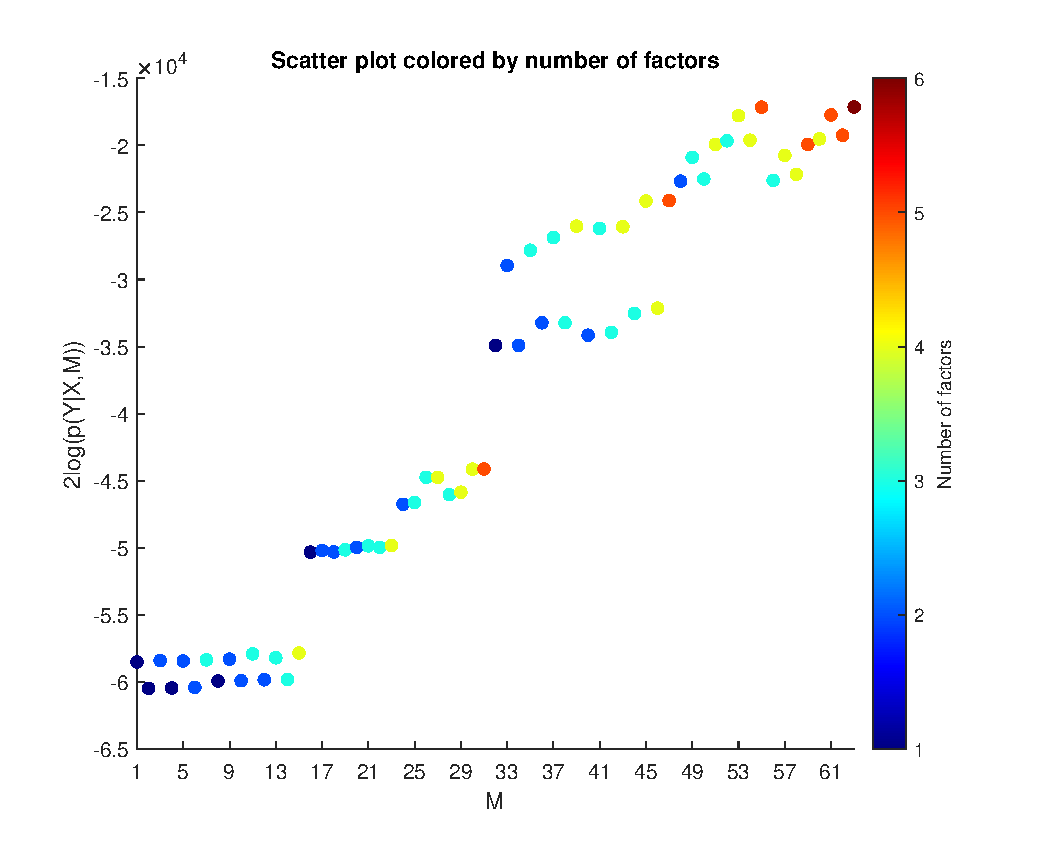
\includegraphics[width=\textwidth]{model_selection.eps}     
    \caption{Log likelihood for every possible value for M}
    % \label{fig:eps-figure}
\end{figure}

Given those values, we conclude that $M^*=63$, which means we should keep all 6 the factors. Probably there is some numerical mistake in calculations due to the limited perdition of floating numbers and the actual maximum value for the likelihood is for $M=55$ which has only 5 factors. 

\section*{Problem 3}

\subsection*{Step 1: Definitions and Notation}

Let the observed classifications from the table be represented as counts:
\[
\mu^a = (\mu^a_1, \mu^a_2, \mu^a_3), \quad \mu^b = (\mu^b_1, \mu^b_2, \mu^b_3), \quad \mu^c = (\mu^c_1, \mu^c_2, \mu^c_3)
\]
where \(\mu^a, \mu^b, \mu^c\) are the counts of categories \(1, 2, 3\) for Persons 1, 2, and 3, respectively.

Using the provided table, we get:
\[
\mu^a = (13, 3, 4), \quad \mu^b = (4, 9, 7), \quad \mu^c = (8, 8, 4)
\]

The combined counts are:
\[
\mu_{\text{total}} = \mu^a + \mu^b + \mu^c = (25,20,15)
\]

The Dirichlet normalization constant is:
\[
Z(u) = \frac{\prod_q \Gamma(u_q)}{\Gamma\left(\sum_q u_q\right)}
\]
Assuming a uniform prior on counts (\(u_q = 1\)), this simplifies to:
\[
Z(u) = \frac{\prod_q \Gamma(1)}{\Gamma(3)} = \frac{1}{2}
\]

\subsection*{Step 2: Likelihoods of the Models}

1. Likelihood for \(H_{\text{indep}}\):
\[
p(o_a, o_b, o_c \mid H_{\text{indep}}) = p(H_{\text{indep}}) \cdot \frac{Z(u + \mu^a)}{Z(u)} \cdot \frac{Z(u + \mu^b)}{Z(u)} \cdot \frac{Z(u + \mu^c)}{Z(u)}
\]

2. Likelihood for \(H_{\text{same}}\):
\[
p(o_a, o_b, o_c \mid H_{\text{same}}) = p(H_{\text{same}}) \cdot \frac{Z(u + \mu_{\text{total}})}{Z(u)}
\]

\subsection*{Step 3: Bayes Factor}
Assuming no prior preference amongst hypotheses, the Bayes factor is:
\[
\text{Bayes Factor} = \frac{p(o_a, o_b, o_c \mid H_{\text{indep}})}{p(o_a, o_b, o_c \mid H_{\text{same}})} = 
\frac{\frac{Z(u + \mu^a)}{Z(u)} \cdot \frac{Z(u + \mu^b)}{Z(u)} \cdot \frac{Z(u + \mu^c)}{Z(u)}}{\frac{Z(u + \mu_{\text{total}})}{Z(u)}}
\]

Simplify:
\[
\text{Bayes Factor} = \frac{Z(u + \mu^a) \cdot Z(u + \mu^b) \cdot Z(u + \mu^c)}{Z(u + \mu_{\text{total}})  \cdot Z(u) \cdot Z(u) }
\]

\subsection*{Step 4: Substitution of Counts and Evaluation}

For the evaluation, the MATLAB script \textit{P3\_hypotheses\_test.m} was used, which gives the result of:

\[
\text{Bayes Factor} = 2.7586
\]

\section*{Problem 4: Mixture Model}

\subsection*{a) Posterior Probability}
The posterior probability that a sample \( x \) was generated from \( f_1(x) \) is computed using Bayes' rule:
\[
P(f_1 | x) = \frac{P(f_1) \cdot P(x | f_1)}{P(x)} = \frac{\theta f_1(x)}{\theta f_1(x) + (1 - \theta) f_2(x)}
\]

\subsection*{ b) Log-Likelihood Using Indicator Function}
Let \( \mathbb{I}(c_i = 1) \) and \( \mathbb{I}(c_i = 0) \) denote indicator functions, where:
\[
\mathbb{I}(c_i = 1) =
\begin{cases}
1, & \text{if } c_i = 1, \\
0, & \text{otherwise}
\end{cases}
\quad
\mathbb{I}(c_i = 0) = 1 - \mathbb{I}(c_i = 1)
\]

The likelihood of the dataset \( \{c_1, x_1, \dots, c_n, x_n\} \) (given i.i.d. coin flips) is:

\[
P(c_1, x_1, \dots, c_n, x_n | \theta) = \prod_{i=1}^n P(c_i, x_i| \theta)
\]

\[
P(c_1, x_1, \dots, c_n, x_n | \theta) = \prod_{i=1}^n \big[ \theta f_1(x_i) \big]^{\mathbb{I}(c_i = 1)} \big[ (1 - \theta) f_2(x_i) \big]^{\mathbb{I}(c_i = 0)}
\]

Taking the natural logarithm, the log-likelihood becomes:
\[
\log P(c_1, x_1, \dots, c_n, x_n | \theta) =
\sum_{i=1}^n \big[ \mathbb{I}(c_i = 1) \log (\theta f_1(x_i)) + \mathbb{I}(c_i = 0) \log ((1 - \theta) f_2(x_i)) \big]
\]

Expanding the terms:
\[
\log P(c_1, x_1, \dots, c_n, x_n | \theta) =
\sum_{i=1}^n \big[ \mathbb{I}(c_i = 1) (\log \theta + \log f_1(x_i)) + \mathbb{I}(c_i = 0) (\log (1 - \theta) + \log f_2(x_i)) \big]
\]

\subsection*{c) Maximum Likelihood Estimator (MLE) for \(\theta\)}
To find the MLE, maximize the log-likelihood with respect to \( \theta \):
\[
\log P(c_1, x_1, \dots, c_n, x_n | \theta) = \sum_{i=1}^n \big[ \mathbb{I}(c_i = 1) \log \theta + \mathbb{I}(c_i = 0) \log (1 - \theta) \big] + \text{(terms independent of } \theta)
\]

Let:
\[
N_1 = \sum_{i=1}^n \mathbb{I}(c_i = 1), \quad N_2 = \sum_{i=1}^n \mathbb{I}(c_i = 0)
\]

Therefore, the  log-likelihood can be rewritten as:
\[
\log P(c_1, x_1, \dots, c_n, x_n | \theta) = N_1 \log \theta + N_2 \log (1 - \theta)
\]

Take the derivative with respect to \( \theta \):
\[
\frac{\partial}{\partial \theta} \big[ N_1 \log \theta + N_2 \log (1 - \theta) \big] = \frac{N_1}{\theta} - \frac{N_2}{1 - \theta}
\]

Set the derivative to zero:
\[
\frac{N_1}{\theta} = \frac{N_2}{1 - \theta}
\]

Solve for \( \theta \):
\[
\theta = \frac{N_1}{N_1 + N_2} = \frac{N_1}{n}  
\]

Thus, the MLE is:
\[
\theta_{\text{MLE}} = \frac{1}{n}  \sum_{i=1}^n \mathbb{I}(c_i = 1)
\]

\section*{Problem 5: EM Algorithm}

\subsection*{E-Step}
Compute the probability that \( x_i \) was generated from \( f_1(x) \) or \( f_2(x) \) , given the current estimate of \( \theta \):
\[
q_{i,1} = P(c_i = 1 | x_i, \theta) = \frac{\theta f_1(x_i)}{\theta f_1(x_i) + (1 - \theta) f_2(x_i)}
\]

\[
q_{i,0} = P(c_i = 0 | x_i, \theta) = \frac{(1 - \theta) f_2(x_i)}{\theta f_1(x_i) + (1 - \theta) f_2(x_i)}
\]

\subsection*{M-Step}

We write the Energy term:
\[
\sum_{i=1}^n  \left\langle  \log P(c_i, x_i| \theta)\right\rangle _{q(c_i \mid x_i , \theta)}
\]
\[
\sum_{i=1}^n  \left\langle  \log P( x_i|c_i, \theta)P( c_i \mid \theta)\right\rangle _{q(c_i \mid x_i , \theta)}
\]

\[
\sum_{i=1}^n  \left\langle  
\log P( x_i|c_i, \theta) +
\log P( c_i \mid \theta)
\right\rangle _{q(c_i \mid x_i , \theta)}
\]

\[
\sum_{i=1}^n    
q_{i,1} \big (\log P( x_i|c_i=1, \theta) +
\log P( c_i =1\mid \theta)\big)+
q_{i,0} \big(\log P( x_i|c_i=0, \theta) +
\log P( c_i=0 \mid \theta) \big)
\]

\[
\sum_{i=1}^n    
q_{i,1} \big (\log f_1( x_i) +
\log  \theta \big)+
q_{i,0} \big(\log f_2( x_i) +
\log ( 1 - \theta) \big)
\]

Let:
\[
Q_1 = \sum_{i=1}^n q_{i,1}, \quad Q_2 = \sum_{i=1}^n q_{i,2}, \quad Q_1 + Q_2 = n
\]
Therefore, we can write it as:
\[
Q_{1} \big (\log f_1( x_i) +
\log  \theta \big)+
Q_{0} \big(\log f_2( x_i) +
\log ( 1 - \theta) \big)
\]
Keeping only the terms dependent on $\theta$ we have:

\[
 Q_1 \log \theta + Q_2 \log (1 - \theta)
\]

Take the derivative with respect to \( \theta \):
\[
\frac{\partial}{\partial \theta} \big[ Q_1 \log \theta + Q_2 \log (1 - \theta) \big] = \frac{Q_1}{\theta} - \frac{Q_2}{1 - \theta}
\]

Set the derivative to zero:
\[
\frac{Q_1}{\theta} = \frac{Q_2}{1 - \theta}
\]

Solve for \( \theta \):
\[
\theta = \frac{Q_1}{Q_1+Q_2} = \frac{Q_1}{n}
\]


\end{document}
